% Options for packages loaded elsewhere
\PassOptionsToPackage{unicode}{hyperref}
\PassOptionsToPackage{hyphens}{url}
%
\documentclass[
]{article}
\usepackage{amsmath,amssymb}
\usepackage{iftex}
\ifPDFTeX
  \usepackage[T1]{fontenc}
  \usepackage[utf8]{inputenc}
  \usepackage{textcomp} % provide euro and other symbols
\else % if luatex or xetex
  \usepackage{unicode-math} % this also loads fontspec
  \defaultfontfeatures{Scale=MatchLowercase}
  \defaultfontfeatures[\rmfamily]{Ligatures=TeX,Scale=1}
\fi
\usepackage{lmodern}
\ifPDFTeX\else
  % xetex/luatex font selection
\fi
% Use upquote if available, for straight quotes in verbatim environments
\IfFileExists{upquote.sty}{\usepackage{upquote}}{}
\IfFileExists{microtype.sty}{% use microtype if available
  \usepackage[]{microtype}
  \UseMicrotypeSet[protrusion]{basicmath} % disable protrusion for tt fonts
}{}
\makeatletter
\@ifundefined{KOMAClassName}{% if non-KOMA class
  \IfFileExists{parskip.sty}{%
    \usepackage{parskip}
  }{% else
    \setlength{\parindent}{0pt}
    \setlength{\parskip}{6pt plus 2pt minus 1pt}}
}{% if KOMA class
  \KOMAoptions{parskip=half}}
\makeatother
\usepackage{xcolor}
\usepackage[margin=1in]{geometry}
\usepackage{color}
\usepackage{fancyvrb}
\newcommand{\VerbBar}{|}
\newcommand{\VERB}{\Verb[commandchars=\\\{\}]}
\DefineVerbatimEnvironment{Highlighting}{Verbatim}{commandchars=\\\{\}}
% Add ',fontsize=\small' for more characters per line
\usepackage{framed}
\definecolor{shadecolor}{RGB}{248,248,248}
\newenvironment{Shaded}{\begin{snugshade}}{\end{snugshade}}
\newcommand{\AlertTok}[1]{\textcolor[rgb]{0.94,0.16,0.16}{#1}}
\newcommand{\AnnotationTok}[1]{\textcolor[rgb]{0.56,0.35,0.01}{\textbf{\textit{#1}}}}
\newcommand{\AttributeTok}[1]{\textcolor[rgb]{0.13,0.29,0.53}{#1}}
\newcommand{\BaseNTok}[1]{\textcolor[rgb]{0.00,0.00,0.81}{#1}}
\newcommand{\BuiltInTok}[1]{#1}
\newcommand{\CharTok}[1]{\textcolor[rgb]{0.31,0.60,0.02}{#1}}
\newcommand{\CommentTok}[1]{\textcolor[rgb]{0.56,0.35,0.01}{\textit{#1}}}
\newcommand{\CommentVarTok}[1]{\textcolor[rgb]{0.56,0.35,0.01}{\textbf{\textit{#1}}}}
\newcommand{\ConstantTok}[1]{\textcolor[rgb]{0.56,0.35,0.01}{#1}}
\newcommand{\ControlFlowTok}[1]{\textcolor[rgb]{0.13,0.29,0.53}{\textbf{#1}}}
\newcommand{\DataTypeTok}[1]{\textcolor[rgb]{0.13,0.29,0.53}{#1}}
\newcommand{\DecValTok}[1]{\textcolor[rgb]{0.00,0.00,0.81}{#1}}
\newcommand{\DocumentationTok}[1]{\textcolor[rgb]{0.56,0.35,0.01}{\textbf{\textit{#1}}}}
\newcommand{\ErrorTok}[1]{\textcolor[rgb]{0.64,0.00,0.00}{\textbf{#1}}}
\newcommand{\ExtensionTok}[1]{#1}
\newcommand{\FloatTok}[1]{\textcolor[rgb]{0.00,0.00,0.81}{#1}}
\newcommand{\FunctionTok}[1]{\textcolor[rgb]{0.13,0.29,0.53}{\textbf{#1}}}
\newcommand{\ImportTok}[1]{#1}
\newcommand{\InformationTok}[1]{\textcolor[rgb]{0.56,0.35,0.01}{\textbf{\textit{#1}}}}
\newcommand{\KeywordTok}[1]{\textcolor[rgb]{0.13,0.29,0.53}{\textbf{#1}}}
\newcommand{\NormalTok}[1]{#1}
\newcommand{\OperatorTok}[1]{\textcolor[rgb]{0.81,0.36,0.00}{\textbf{#1}}}
\newcommand{\OtherTok}[1]{\textcolor[rgb]{0.56,0.35,0.01}{#1}}
\newcommand{\PreprocessorTok}[1]{\textcolor[rgb]{0.56,0.35,0.01}{\textit{#1}}}
\newcommand{\RegionMarkerTok}[1]{#1}
\newcommand{\SpecialCharTok}[1]{\textcolor[rgb]{0.81,0.36,0.00}{\textbf{#1}}}
\newcommand{\SpecialStringTok}[1]{\textcolor[rgb]{0.31,0.60,0.02}{#1}}
\newcommand{\StringTok}[1]{\textcolor[rgb]{0.31,0.60,0.02}{#1}}
\newcommand{\VariableTok}[1]{\textcolor[rgb]{0.00,0.00,0.00}{#1}}
\newcommand{\VerbatimStringTok}[1]{\textcolor[rgb]{0.31,0.60,0.02}{#1}}
\newcommand{\WarningTok}[1]{\textcolor[rgb]{0.56,0.35,0.01}{\textbf{\textit{#1}}}}
\usepackage{graphicx}
\makeatletter
\def\maxwidth{\ifdim\Gin@nat@width>\linewidth\linewidth\else\Gin@nat@width\fi}
\def\maxheight{\ifdim\Gin@nat@height>\textheight\textheight\else\Gin@nat@height\fi}
\makeatother
% Scale images if necessary, so that they will not overflow the page
% margins by default, and it is still possible to overwrite the defaults
% using explicit options in \includegraphics[width, height, ...]{}
\setkeys{Gin}{width=\maxwidth,height=\maxheight,keepaspectratio}
% Set default figure placement to htbp
\makeatletter
\def\fps@figure{htbp}
\makeatother
\setlength{\emergencystretch}{3em} % prevent overfull lines
\providecommand{\tightlist}{%
  \setlength{\itemsep}{0pt}\setlength{\parskip}{0pt}}
\setcounter{secnumdepth}{-\maxdimen} % remove section numbering
\usepackage{booktabs}
\ifLuaTeX
  \usepackage{selnolig}  % disable illegal ligatures
\fi
\IfFileExists{bookmark.sty}{\usepackage{bookmark}}{\usepackage{hyperref}}
\IfFileExists{xurl.sty}{\usepackage{xurl}}{} % add URL line breaks if available
\urlstyle{same}
\hypersetup{
  pdftitle={HW3\_yc4384\_Cynthia},
  pdfauthor={Yangyang Chen},
  hidelinks,
  pdfcreator={LaTeX via pandoc}}

\title{HW3\_yc4384\_Cynthia}
\author{Yangyang Chen}
\date{2024-02-29}

\begin{document}
\maketitle

\hypertarget{problem-1}{%
\subsection{Problem 1}\label{problem-1}}

\hypertarget{a-fit-a-prospective-model-to-the-data-to-study-the-relation-between-alcohol-consumption-age-and-disease-model-age-as-a-continuous-variable-taking-values-25-35-45-55-65-and-75.-interpret-the-result.}{%
\subsubsection{(a) Fit a prospective model to the data to study the
relation between alcohol consumption, age, and disease (model age as a
continuous variable taking values 25, 35, 45, 55, 65, and 75). Interpret
the
result.}\label{a-fit-a-prospective-model-to-the-data-to-study-the-relation-between-alcohol-consumption-age-and-disease-model-age-as-a-continuous-variable-taking-values-25-35-45-55-65-and-75.-interpret-the-result.}}

Using logistics regression model to fit data from prospective study:

\[log(\frac{\pi}{1-\pi}) = \beta_0 +\beta_1X_{alc}+\beta_2X_{age}\]

\begin{Shaded}
\begin{Highlighting}[]
\CommentTok{\# load data}
\NormalTok{age }\OtherTok{=} \FunctionTok{seq}\NormalTok{(}\AttributeTok{from =} \DecValTok{25}\NormalTok{, }\AttributeTok{to =} \DecValTok{75}\NormalTok{, }\AttributeTok{by =} \DecValTok{10}\NormalTok{) }\SpecialCharTok{|\textgreater{}} 
  \FunctionTok{rep}\NormalTok{(}\DecValTok{2}\NormalTok{)}
\NormalTok{case }\OtherTok{=} \FunctionTok{c}\NormalTok{(}\DecValTok{1}\NormalTok{, }\DecValTok{4}\NormalTok{, }\DecValTok{25}\NormalTok{, }\DecValTok{42}\NormalTok{, }\DecValTok{19}\NormalTok{, }\DecValTok{5}\NormalTok{, }\DecValTok{0}\NormalTok{, }\DecValTok{5}\NormalTok{, }\DecValTok{21}\NormalTok{, }\DecValTok{34}\NormalTok{, }\DecValTok{36}\NormalTok{, }\DecValTok{8}\NormalTok{)}
\NormalTok{control }\OtherTok{=} \FunctionTok{c}\NormalTok{(}\DecValTok{9}\NormalTok{, }\DecValTok{26}\NormalTok{, }\DecValTok{29}\NormalTok{, }\DecValTok{27}\NormalTok{, }\DecValTok{18}\NormalTok{, }\DecValTok{0}\NormalTok{, }\DecValTok{106}\NormalTok{, }\DecValTok{164}\NormalTok{, }\DecValTok{138}\NormalTok{, }\DecValTok{139}\NormalTok{, }\DecValTok{88}\NormalTok{, }\DecValTok{31}\NormalTok{)}
\NormalTok{alc }\OtherTok{=} \FunctionTok{c}\NormalTok{(}\FunctionTok{rep}\NormalTok{(}\DecValTok{1}\NormalTok{,}\DecValTok{6}\NormalTok{), }\FunctionTok{rep}\NormalTok{(}\DecValTok{0}\NormalTok{, }\DecValTok{6}\NormalTok{))}
\NormalTok{resp }\OtherTok{=} \FunctionTok{cbind}\NormalTok{(case, control)}

\CommentTok{\# Model fitting using logit link}
\NormalTok{glm\_logit}\OtherTok{=}\FunctionTok{glm}\NormalTok{(resp }\SpecialCharTok{\textasciitilde{}}\NormalTok{ alc }\SpecialCharTok{+}\NormalTok{ age, }\AttributeTok{family=}\FunctionTok{binomial}\NormalTok{(}\AttributeTok{link=}\StringTok{\textquotesingle{}logit\textquotesingle{}}\NormalTok{))}
\FunctionTok{summary}\NormalTok{(glm\_logit)}
\end{Highlighting}
\end{Shaded}

\begin{verbatim}
## 
## Call:
## glm(formula = resp ~ alc + age, family = binomial(link = "logit"))
## 
## Coefficients:
##              Estimate Std. Error z value Pr(>|z|)    
## (Intercept) -5.023449   0.418224 -12.011   <2e-16 ***
## alc          1.780000   0.187086   9.514   <2e-16 ***
## age          0.061579   0.007291   8.446   <2e-16 ***
## ---
## Signif. codes:  0 '***' 0.001 '**' 0.01 '*' 0.05 '.' 0.1 ' ' 1
## 
## (Dispersion parameter for binomial family taken to be 1)
## 
##     Null deviance: 211.608  on 11  degrees of freedom
## Residual deviance:  31.932  on  9  degrees of freedom
## AIC: 78.259
## 
## Number of Fisher Scoring iterations: 4
\end{verbatim}

Hence, the logistics regression model is:
\[log(\frac{\pi}{1-\pi}) = -5.02 + 1.78X_{alc} + 0.06*X_{age}\]

Interpretation:

\begin{itemize}
\item
  The model suggests a significant relationship between esophageal
  cancer, daily alcohol consumption adjusted and age.
\item
  \(\beta_{1}\): the log odds ratio of having the disease among heavy
  drinkers is \(1.78\) times the odds odds ratio of non-heavy drinkers,
  keeping age fixed.
\item
  \(exp(\beta_{1})\): odds ratio for the association between disease and
  alcohol consumption, holding age constant.
\item
  \(\beta_{2}\): the log odds ratio of having the disease will increase
  by \(0.06\) for every unit increment in age, keeping alcohol
  consumption fixed.
\item
  \(exp(\beta_{2})\): the odds ratio for the association between disease
  and age, holding alcohol consumption constant.
\item
  This model appears to fit the data well, as indicated by the
  significant coefficients and the reduction in deviance from the null
  model to the fitted model.
\end{itemize}

\begin{enumerate}
\def\labelenumi{(\alph{enumi})}
\setcounter{enumi}{1}
\tightlist
\item
\end{enumerate}

\begin{Shaded}
\begin{Highlighting}[]
\NormalTok{age }\OtherTok{=} \FunctionTok{c}\NormalTok{(}\DecValTok{1}\SpecialCharTok{:}\DecValTok{6}\NormalTok{) }\SpecialCharTok{|\textgreater{}} 
  \FunctionTok{factor}\NormalTok{()}
\NormalTok{ind }\OtherTok{=} \FunctionTok{dummy.code}\NormalTok{(age)}
\NormalTok{grp1 }\OtherTok{=} \FunctionTok{rep}\NormalTok{(ind[,}\DecValTok{1}\NormalTok{],}\DecValTok{2}\NormalTok{)}
\NormalTok{grp2 }\OtherTok{=} \FunctionTok{rep}\NormalTok{(ind[,}\DecValTok{2}\NormalTok{],}\DecValTok{2}\NormalTok{)}
\NormalTok{grp3 }\OtherTok{=} \FunctionTok{rep}\NormalTok{(ind[,}\DecValTok{3}\NormalTok{],}\DecValTok{2}\NormalTok{)}
\NormalTok{grp4 }\OtherTok{=} \FunctionTok{rep}\NormalTok{(ind[,}\DecValTok{4}\NormalTok{],}\DecValTok{2}\NormalTok{)}
\NormalTok{grp5 }\OtherTok{=} \FunctionTok{rep}\NormalTok{(ind[,}\DecValTok{5}\NormalTok{],}\DecValTok{2}\NormalTok{)}
\NormalTok{grp6 }\OtherTok{=} \FunctionTok{rep}\NormalTok{(ind[,}\DecValTok{6}\NormalTok{],}\DecValTok{2}\NormalTok{)}

\NormalTok{M\_0 }\OtherTok{=} \FunctionTok{glm}\NormalTok{(resp }\SpecialCharTok{\textasciitilde{}}\NormalTok{ grp1 }\SpecialCharTok{+}\NormalTok{ grp2 }\SpecialCharTok{+}\NormalTok{ grp3 }\SpecialCharTok{+}\NormalTok{ grp4 }\SpecialCharTok{+}\NormalTok{ grp5 }\SpecialCharTok{+}\NormalTok{ grp6, }\AttributeTok{family =} \FunctionTok{binomial}\NormalTok{(}\AttributeTok{link =} \StringTok{\textquotesingle{}logit\textquotesingle{}}\NormalTok{))}
\FunctionTok{summary}\NormalTok{(M\_0)}
\end{Highlighting}
\end{Shaded}

\begin{verbatim}
## 
## Call:
## glm(formula = resp ~ grp1 + grp2 + grp3 + grp4 + grp5 + grp6, 
##     family = binomial(link = "logit"))
## 
## Coefficients: (1 not defined because of singularities)
##             Estimate Std. Error z value Pr(>|z|)    
## (Intercept) -0.86904    0.33043  -2.630 0.008537 ** 
## grp1        -3.87589    1.05728  -3.666 0.000246 ***
## grp2        -2.18076    0.47493  -4.592 4.39e-06 ***
## grp3        -0.42031    0.37001  -1.136 0.255977    
## grp4         0.08778    0.35828   0.245 0.806445    
## grp5         0.21293    0.36986   0.576 0.564812    
## grp6              NA         NA      NA       NA    
## ---
## Signif. codes:  0 '***' 0.001 '**' 0.01 '*' 0.05 '.' 0.1 ' ' 1
## 
## (Dispersion parameter for binomial family taken to be 1)
## 
##     Null deviance: 211.608  on 11  degrees of freedom
## Residual deviance:  90.563  on  6  degrees of freedom
## AIC: 142.89
## 
## Number of Fisher Scoring iterations: 6
\end{verbatim}

\begin{Shaded}
\begin{Highlighting}[]
\NormalTok{dev\_m0 }\OtherTok{=} \FunctionTok{residuals}\NormalTok{(M\_0, }\AttributeTok{type =} \StringTok{"deviance"}\NormalTok{)}\SpecialCharTok{\^{}}\DecValTok{2} \SpecialCharTok{|\textgreater{}} \FunctionTok{sum}\NormalTok{()}

\NormalTok{M\_1 }\OtherTok{=} \FunctionTok{glm}\NormalTok{(resp }\SpecialCharTok{\textasciitilde{}}\NormalTok{ alc }\SpecialCharTok{+}\NormalTok{ grp1 }\SpecialCharTok{+}\NormalTok{ grp2 }\SpecialCharTok{+}\NormalTok{ grp3 }\SpecialCharTok{+}\NormalTok{ grp4 }\SpecialCharTok{+}\NormalTok{ grp5 }\SpecialCharTok{+}\NormalTok{ grp6, }\AttributeTok{family =} \FunctionTok{binomial}\NormalTok{(}\AttributeTok{link =} \StringTok{\textquotesingle{}logit\textquotesingle{}}\NormalTok{))}
\FunctionTok{summary}\NormalTok{(M\_1)}
\end{Highlighting}
\end{Shaded}

\begin{verbatim}
## 
## Call:
## glm(formula = resp ~ alc + grp1 + grp2 + grp3 + grp4 + grp5 + 
##     grp6, family = binomial(link = "logit"))
## 
## Coefficients: (1 not defined because of singularities)
##              Estimate Std. Error z value Pr(>|z|)    
## (Intercept) -1.092158   0.344216  -3.173 0.001509 ** 
## alc          1.669890   0.189602   8.807  < 2e-16 ***
## grp1        -3.962190   1.065035  -3.720 0.000199 ***
## grp2        -2.419896   0.491328  -4.925 8.43e-07 ***
## grp3        -0.763428   0.389837  -1.958 0.050192 .  
## grp4        -0.248700   0.376735  -0.660 0.509161    
## grp5         0.004692   0.387043   0.012 0.990328    
## grp6               NA         NA      NA       NA    
## ---
## Signif. codes:  0 '***' 0.001 '**' 0.01 '*' 0.05 '.' 0.1 ' ' 1
## 
## (Dispersion parameter for binomial family taken to be 1)
## 
##     Null deviance: 211.608  on 11  degrees of freedom
## Residual deviance:  11.041  on  5  degrees of freedom
## AIC: 65.369
## 
## Number of Fisher Scoring iterations: 5
\end{verbatim}

\begin{Shaded}
\begin{Highlighting}[]
\CommentTok{\# Define the data}
\NormalTok{Model }\OtherTok{\textless{}{-}} \FunctionTok{c}\NormalTok{(}\StringTok{"$M\_0$"}\NormalTok{, }\StringTok{"$M\_1$"}\NormalTok{)}
\NormalTok{Linear\_predictor }\OtherTok{\textless{}{-}} \FunctionTok{c}\NormalTok{(}\StringTok{"$}\SpecialCharTok{\textbackslash{}\textbackslash{}}\StringTok{alpha\_j$"}\NormalTok{, }\StringTok{"$}\SpecialCharTok{\textbackslash{}\textbackslash{}}\StringTok{alpha\_j + }\SpecialCharTok{\textbackslash{}\textbackslash{}}\StringTok{beta X$"}\NormalTok{)}
\NormalTok{Deviance }\OtherTok{\textless{}{-}} \FunctionTok{c}\NormalTok{(}\FloatTok{90.56}\NormalTok{, }\FloatTok{11.04}\NormalTok{)}
\NormalTok{df }\OtherTok{\textless{}{-}} \FunctionTok{c}\NormalTok{(}\DecValTok{6}\NormalTok{, }\DecValTok{5}\NormalTok{)}

\CommentTok{\# Create a data frame}
\NormalTok{outp }\OtherTok{\textless{}{-}} \FunctionTok{data.frame}\NormalTok{(Model, Linear\_predictor, Deviance, df, }\AttributeTok{stringsAsFactors =} \ConstantTok{FALSE}\NormalTok{)}

\CommentTok{\# Set column names}
\FunctionTok{colnames}\NormalTok{(outp) }\OtherTok{\textless{}{-}} \FunctionTok{c}\NormalTok{(}\StringTok{"Model"}\NormalTok{, }\StringTok{"Linear Predictor"}\NormalTok{, }\StringTok{"Deviance"}\NormalTok{, }\StringTok{"df"}\NormalTok{)}

\CommentTok{\# Print the data frame using knitr::kable() with format = "latex" and escape = FALSE}

\NormalTok{knitr}\SpecialCharTok{::}\FunctionTok{kable}\NormalTok{(outp, }\AttributeTok{format =} \StringTok{"latex"}\NormalTok{, }\AttributeTok{escape =} \ConstantTok{FALSE}\NormalTok{, }\AttributeTok{align =} \StringTok{"c"}\NormalTok{, }\AttributeTok{booktabs =} \ConstantTok{TRUE}\NormalTok{)}
\end{Highlighting}
\end{Shaded}

\begin{tabular}{cccc}
\toprule
Model & Linear Predictor & Deviance & df\\
\midrule
$M_0$ & $\alpha_j$ & 90.56 & 6\\
$M_1$ & $\alpha_j + \beta X$ & 11.04 & 5\\
\bottomrule
\end{tabular}

Hypothesis Testing:

\[H_0: \beta_{alc}=0 \\ \ H_1:\beta_{alc} \ne 0 \]
\[stat = 79.52 \sim \chi^2_{1}\] \[p-value <0.0001\]

Hence, we reject the null hypothesis and we have sufficient evidence to
conlcude that there's an significant association between disease and
alcohol consumption.

\hypertarget{problem-2}{%
\subsection{Problem 2}\label{problem-2}}

\hypertarget{a-fit-a-logistic-regression-model-to-study-the-relation-between-germination-rates-and-different-types-of-seed-and-root-extract.-interpret-the-result.}{%
\subsubsection{(a) Fit a logistic regression model to study the relation
between germination rates and different types of seed and root extract.
Interpret the
result.}\label{a-fit-a-logistic-regression-model-to-study-the-relation-between-germination-rates-and-different-types-of-seed-and-root-extract.-interpret-the-result.}}

Let \(Y_i\) denote the number of seeds germinates among \(m_i\) seeds
with the \(ith\) covariate pattern. The logistic regression model:

\[log(\frac{\pi}{1-\pi}) = \beta_0 + \beta_1X_{seed}+\beta_2X_{root};\]

\begin{Shaded}
\begin{Highlighting}[]
\CommentTok{\# input data}
\NormalTok{x}\OtherTok{=}\FunctionTok{c}\NormalTok{(}\FunctionTok{rep}\NormalTok{(}\DecValTok{1}\NormalTok{,}\DecValTok{10}\NormalTok{),}\FunctionTok{rep}\NormalTok{(}\DecValTok{0}\NormalTok{,}\DecValTok{11}\NormalTok{)) }\CommentTok{\# roots category}
\NormalTok{z}\OtherTok{=}\FunctionTok{c}\NormalTok{(}\FunctionTok{rep}\NormalTok{(}\DecValTok{1}\NormalTok{,}\DecValTok{5}\NormalTok{), }\FunctionTok{rep}\NormalTok{(}\DecValTok{0}\NormalTok{,}\DecValTok{6}\NormalTok{), }\FunctionTok{rep}\NormalTok{(}\DecValTok{1}\NormalTok{,}\DecValTok{5}\NormalTok{), }\FunctionTok{rep}\NormalTok{(}\DecValTok{0}\NormalTok{,}\DecValTok{5}\NormalTok{)) }\CommentTok{\# seeds category}
\NormalTok{y}\OtherTok{=}\FunctionTok{c}\NormalTok{(}\DecValTok{10}\NormalTok{,}\DecValTok{23}\NormalTok{,}\DecValTok{23}\NormalTok{,}\DecValTok{26}\NormalTok{,}\DecValTok{17}\NormalTok{,}\DecValTok{8}\NormalTok{,}\DecValTok{10}\NormalTok{,}\DecValTok{8}\NormalTok{,}\DecValTok{23}\NormalTok{,}\DecValTok{0}\NormalTok{,}\DecValTok{5}\NormalTok{,}\DecValTok{53}\NormalTok{,}\DecValTok{55}\NormalTok{,}\DecValTok{32}\NormalTok{,}\DecValTok{46}\NormalTok{,}\DecValTok{10}\NormalTok{,}\DecValTok{3}\NormalTok{,}\DecValTok{22}\NormalTok{,}\DecValTok{15}\NormalTok{,}\DecValTok{32}\NormalTok{,}\DecValTok{3}\NormalTok{) }\CommentTok{\# survive=1}
\NormalTok{m}\OtherTok{=}\FunctionTok{c}\NormalTok{(}\DecValTok{39}\NormalTok{,}\DecValTok{62}\NormalTok{,}\DecValTok{81}\NormalTok{,}\DecValTok{51}\NormalTok{,}\DecValTok{39}\NormalTok{,}\DecValTok{16}\NormalTok{,}\DecValTok{30}\NormalTok{,}\DecValTok{28}\NormalTok{,}\DecValTok{45}\NormalTok{,}\DecValTok{4}\NormalTok{,}\DecValTok{6}\NormalTok{,}\DecValTok{74}\NormalTok{,}\DecValTok{72}\NormalTok{,}\DecValTok{51}\NormalTok{,}\DecValTok{79}\NormalTok{,}\DecValTok{13}\NormalTok{,}\DecValTok{12}\NormalTok{,}\DecValTok{41}\NormalTok{,}\DecValTok{30}\NormalTok{,}\DecValTok{51}\NormalTok{,}\DecValTok{7}\NormalTok{)}
\NormalTok{data}\OtherTok{=}\FunctionTok{data.frame}\NormalTok{(x,y,m)}
\FunctionTok{plot}\NormalTok{(x,m)}
\end{Highlighting}
\end{Shaded}

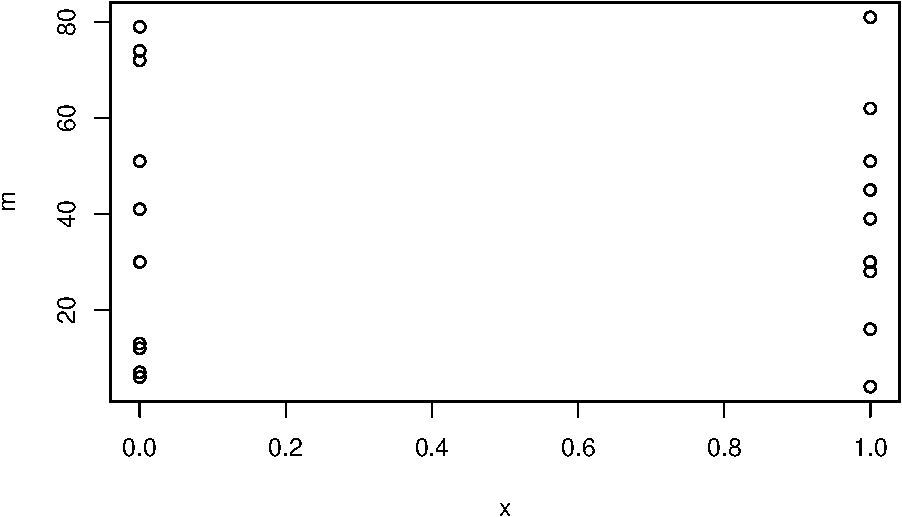
\includegraphics{yc4384_hw3_files/figure-latex/unnamed-chunk-3-1.pdf}

\begin{Shaded}
\begin{Highlighting}[]
\FunctionTok{plot}\NormalTok{(y,m)}
\end{Highlighting}
\end{Shaded}

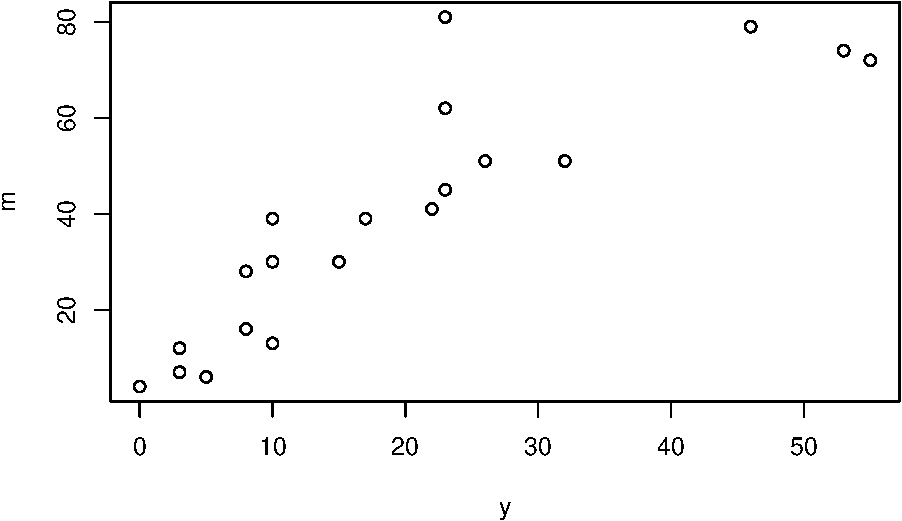
\includegraphics{yc4384_hw3_files/figure-latex/unnamed-chunk-3-2.pdf}

\begin{Shaded}
\begin{Highlighting}[]
\FunctionTok{summary}\NormalTok{(m}\SpecialCharTok{{-}}\NormalTok{y) }\DocumentationTok{\#\# m \textgreater{}= y}
\end{Highlighting}
\end{Shaded}

\begin{verbatim}
##    Min. 1st Qu.  Median    Mean 3rd Qu.    Max. 
##    1.00    9.00   19.00   19.38   22.00   58.00
\end{verbatim}

\begin{Shaded}
\begin{Highlighting}[]
\CommentTok{\# fit binomial (logistic) without dispersion}
\NormalTok{none.disp}\OtherTok{=}\FunctionTok{glm}\NormalTok{(}\FunctionTok{cbind}\NormalTok{(y,m}\SpecialCharTok{{-}}\NormalTok{y)}\SpecialCharTok{\textasciitilde{}}\NormalTok{x}\SpecialCharTok{+}\NormalTok{z, }\AttributeTok{family=}\FunctionTok{binomial}\NormalTok{(}\AttributeTok{link=}\StringTok{\textquotesingle{}logit\textquotesingle{}}\NormalTok{))}
\FunctionTok{summary}\NormalTok{(none.disp)}
\end{Highlighting}
\end{Shaded}

\begin{verbatim}
## 
## Call:
## glm(formula = cbind(y, m - y) ~ x + z, family = binomial(link = "logit"))
## 
## Coefficients:
##             Estimate Std. Error z value Pr(>|z|)    
## (Intercept)   0.3884     0.1410   2.755  0.00588 ** 
## x            -1.0668     0.1442  -7.396  1.4e-13 ***
## z             0.2391     0.1538   1.555  0.12004    
## ---
## Signif. codes:  0 '***' 0.001 '**' 0.01 '*' 0.05 '.' 0.1 ' ' 1
## 
## (Dispersion parameter for binomial family taken to be 1)
## 
##     Null deviance: 98.719  on 20  degrees of freedom
## Residual deviance: 40.328  on 18  degrees of freedom
## AIC: 122.92
## 
## Number of Fisher Scoring iterations: 4
\end{verbatim}

\begin{Shaded}
\begin{Highlighting}[]
\NormalTok{G.stat}\OtherTok{=}\FunctionTok{sum}\NormalTok{(}\FunctionTok{residuals}\NormalTok{(none.disp,}\AttributeTok{type=}\StringTok{\textquotesingle{}pearson\textquotesingle{}}\NormalTok{)}\SpecialCharTok{\^{}}\DecValTok{2}\NormalTok{) }\CommentTok{\# pearson chisq }
\NormalTok{G.stat}
\end{Highlighting}
\end{Shaded}

\begin{verbatim}
## [1] 38.8492
\end{verbatim}

The binomial logistic without dispersion was fitted with the following
results:

\[log(\frac{\pi}{1-\pi}) = 0.3884 - 1.0668*X_{root}+0.2391*X_{seed}\]

Interpretation:

\[\hat{b_0} = 0.3884,\ standard \ error(b_0) = 0.1410;\]

\begin{itemize}
\tightlist
\item
  The log odds ratio of a O.aegyptiaca 73 seed grown in cucumber extract
  for germinating is 0.38.
\end{itemize}

\[\hat{b_1} = 0.2391,\ standard \ error(b_1) = 0.1538;\]

\begin{itemize}
\tightlist
\item
  The estimated log odds ratio for comparing O.aegyptiaca 75 seeds and
  O.aegyptiaca 73 seeds, holding root extract fixed is 0.2391.
\end{itemize}

\[\hat{b_2} = -1.0668,\ standard \ error(b_2) = 0.1442;\]

\begin{itemize}
\tightlist
\item
  The estimated odds ratio for comparing bean and cucumber extract
  amongst O.aegyptiaca 73 seeds, holding seed species fixed is -1.0668.
\end{itemize}

\[Pearson-\chi^2 statistic: X^2 = \sum X_i^2 = 41.226 \ and\ Deviance \ D = \sum d_i^2 = 40.328.\]

\begin{Shaded}
\begin{Highlighting}[]
\CommentTok{\# goodness of fit}
\NormalTok{pval}\OtherTok{=}\DecValTok{1}\SpecialCharTok{{-}}\FunctionTok{pchisq}\NormalTok{(none.disp}\SpecialCharTok{$}\NormalTok{deviance,}\DecValTok{21{-}3}\NormalTok{) }
\NormalTok{pval }\CommentTok{\# bad fit, reject the fitting}
\end{Highlighting}
\end{Shaded}

\begin{verbatim}
## [1] 0.001882762
\end{verbatim}

\begin{itemize}
\tightlist
\item
  Comparing \(X^2\) and \(D\) with \(\chi^2(18)\), we concluded that the
  model appears to fit bad.
\end{itemize}

\hypertarget{b-is-there-over-dispersion-if-so-what-is-the-estimate-of-dispersion-parameter-update-your-model-and-reinterpret-the-result.}{%
\subsubsection{(b) Is there over dispersion? If so, what is the estimate
of dispersion parameter? Update your model and reinterpret the
result.}\label{b-is-there-over-dispersion-if-so-what-is-the-estimate-of-dispersion-parameter-update-your-model-and-reinterpret-the-result.}}

Estimating the dispersion parameter by following two methods:

First,\[\hat{\phi} = G_0/(n-p),\] where
\[G_0 = \sum_{i=1}^{n}{\frac{(y_i-m_i \hat{\pi_i})^2}{m_i\hat{\pi_i}(1-\hat{\pi_i})\phi}} \sim \chi^2(n-p)\ \]
is the generalized Pearson \(\chi^2\) from the original model fitting
without over-dispersion.

Second, \[\hat{\phi} = \frac{D_0}{n-p}\]

\begin{Shaded}
\begin{Highlighting}[]
\CommentTok{\# calc dispersion para in 2 methods}
\CommentTok{\# the first method}
\NormalTok{phi}\OtherTok{=}\NormalTok{G.stat}\SpecialCharTok{/}\NormalTok{(}\DecValTok{21{-}3}\NormalTok{)}
\NormalTok{phi}
\end{Highlighting}
\end{Shaded}

\begin{verbatim}
## [1] 2.158289
\end{verbatim}

\begin{Shaded}
\begin{Highlighting}[]
\CommentTok{\# the second method}
\NormalTok{tilde.phi}\OtherTok{=}\NormalTok{none.disp}\SpecialCharTok{$}\NormalTok{deviance}\SpecialCharTok{/}\NormalTok{none.disp}\SpecialCharTok{$}\NormalTok{df.residual}
\NormalTok{tilde.phi }\CommentTok{\# similar to the one estimated from pearson chisq }
\end{Highlighting}
\end{Shaded}

\begin{verbatim}
## [1] 2.240455
\end{verbatim}

\begin{Shaded}
\begin{Highlighting}[]
\CommentTok{\# test over{-}dispersion (half normal plot)}
\NormalTok{res}\OtherTok{=}\FunctionTok{residuals}\NormalTok{(none.disp,}\AttributeTok{type=}\StringTok{\textquotesingle{}pearson\textquotesingle{}}\NormalTok{)}
\FunctionTok{plot}\NormalTok{(}\FunctionTok{qnorm}\NormalTok{((}\DecValTok{21}\SpecialCharTok{+}\DecValTok{1}\SpecialCharTok{:}\DecValTok{21}\FloatTok{+0.5}\NormalTok{)}\SpecialCharTok{/}\NormalTok{(}\DecValTok{2}\SpecialCharTok{*}\DecValTok{21}\FloatTok{+1.125}\NormalTok{)),}\FunctionTok{sort}\NormalTok{(}\FunctionTok{abs}\NormalTok{(res)),}\AttributeTok{xlab=}\StringTok{\textquotesingle{}Expected Half{-}Normal Order Stats\textquotesingle{}}\NormalTok{,}\AttributeTok{ylab=}\StringTok{\textquotesingle{}Ordered Abs Pearson Residuals\textquotesingle{}}\NormalTok{)}
\FunctionTok{abline}\NormalTok{(}\AttributeTok{a=}\DecValTok{0}\NormalTok{,}\AttributeTok{b=}\DecValTok{1}\NormalTok{)}
\FunctionTok{abline}\NormalTok{(}\AttributeTok{a=}\DecValTok{0}\NormalTok{,}\AttributeTok{b=}\FunctionTok{sqrt}\NormalTok{(phi),}\AttributeTok{lty=}\DecValTok{2}\NormalTok{, }\AttributeTok{col =} \StringTok{\textquotesingle{}red\textquotesingle{}}\NormalTok{)}
\end{Highlighting}
\end{Shaded}

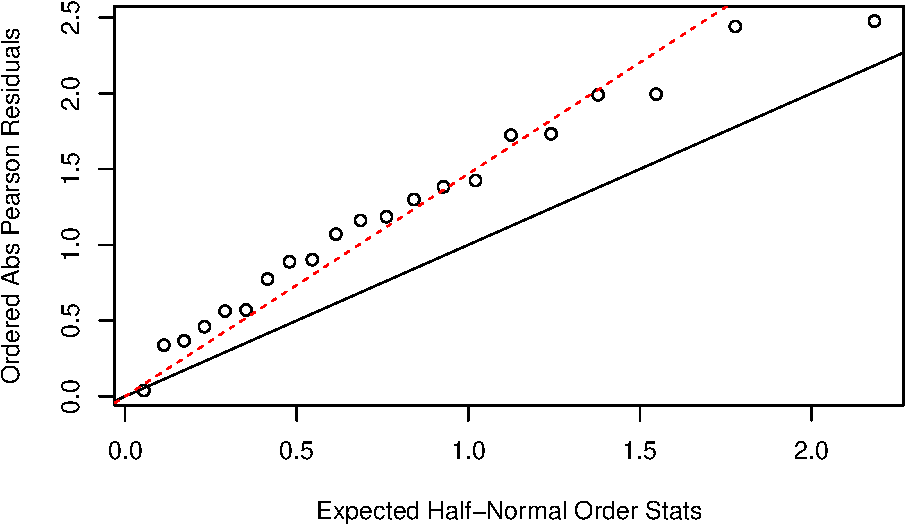
\includegraphics{yc4384_hw3_files/figure-latex/unnamed-chunk-5-1.pdf}

\begin{itemize}
\item
  Therefore, there exists over-dispersion in our model and the estimate
  of dispersion parameter: \(\hat{\phi} = 2.1697\).
\item
  Half-normal plot using residuals from this model shows evidence of
  over-dispersion.
\item
  Next, we updated regression model.
\end{itemize}

\begin{Shaded}
\begin{Highlighting}[]
\CommentTok{\# fit model with constant over{-}dispersion}
\FunctionTok{summary}\NormalTok{(none.disp,}\AttributeTok{dispersion=}\NormalTok{phi)}
\end{Highlighting}
\end{Shaded}

\begin{verbatim}
## 
## Call:
## glm(formula = cbind(y, m - y) ~ x + z, family = binomial(link = "logit"))
## 
## Coefficients:
##             Estimate Std. Error z value Pr(>|z|)    
## (Intercept)   0.3884     0.2071   1.875   0.0608 .  
## x            -1.0668     0.2119  -5.034 4.79e-07 ***
## z             0.2391     0.2259   1.058   0.2900    
## ---
## Signif. codes:  0 '***' 0.001 '**' 0.01 '*' 0.05 '.' 0.1 ' ' 1
## 
## (Dispersion parameter for binomial family taken to be 2.158289)
## 
##     Null deviance: 98.719  on 20  degrees of freedom
## Residual deviance: 40.328  on 18  degrees of freedom
## AIC: 122.92
## 
## Number of Fisher Scoring iterations: 4
\end{verbatim}

The binomial logistic with dispersion was fitted with the following
results: \[b_0 = 0.3884,\ standard \ error(b_1) = 0.2071;\]
\[b_1 = -1.0668,\ standard \ error(b_1) = 0.2119;\]
\[b_2 = 0.2391,\ standard \ error(b_2) = 0.2259;\]
\[Pearson-\chi^2 statistic: X^2 = \sum X_i^2 = 41.226 \ and\ Deviance \ D = \sum d_i^2 = 40.328.\]

\hypertarget{c-what-is-a-plausible-cause-of-the-over-dispersion}{%
\subsubsection{(c) What is a plausible cause of the over
dispersion?}\label{c-what-is-a-plausible-cause-of-the-over-dispersion}}

Since different groups may have different germination rate which follow
the same distribution, the response variables should follows a
beta-binomial distribution rather than binomial distribution.

\end{document}
